%-----------------------------------------------------------------------------
% Schriftgr��e, Layout, Papierformat, Art des Dokumentes
%-----------------------------------------------------------------------------
\documentclass[12pt,					% Grundschriftge
							 oneside,			% einseitiges Dokument
							 a4paper,			% Papiergr��e
							 halfparskip,		% Einzug bei einem Absatz
							 liststotoc,			% Verzeichniss (Abbildungen erc.) in das Inhaltverzeichnis
							 bibtotoc,			% Literaturverzeichnis ins Inhaltverzeichnis
							 fleqn,				% Mathematische Formeln linksb�ndig darstellen
							 pointlessnumbers]	% Punkt am Ende der Nummerierung des Inhaltsverzeichnisses 													entfernen
							 {scrreprt}

%-----------------------------------------------------------------------------
% Konstanten festlegen
%-----------------------------------------------------------------------------
\newcommand{\VerfasserJ}{Josef Prothmann}
\newcommand{\EmailJ}{j.prothmann@stud.hs-wismar.de}
\newcommand{\GeburtstagJ}{16. Dezember 1998}
\newcommand{\GeburtsortJ}{Dannenberg/ Elbe}

\newcommand{\Titel}{QR-Code}
\newcommand{\Betreuer}{Prof. Dr. H. Litschke}



\newcommand{\blankpage}{
%	\newpage
%	\thispagestyle{empty}
%	\mbox{}
	\newpage
}

%-----------------------------------------------------------------------------
% verwendete Pakete
%-----------------------------------------------------------------------------
\usepackage[utf8]{inputenc}		% Zeichkodierung , Umlaute erlauben
\usepackage[T1]{fontenc}				% Wahl des Fonts, bzw. der Kodierung
\usepackage[english,ngerman]{babel}		% neue deutsche Rechtschreibung verwenden
\usepackage{graphicx}					% erm�glicht das Einbinden von Grafiken, sehr wichtig!
\usepackage{fancyhdr}					% f�r formatierte Kopf- und Fu�zeilen
\usepackage{setspace}					% Package zum Kontrollieren von Leerr�umen
\usepackage{subfigure}					% erweiterte Darstellung von Bildern
\usepackage{listings}					% M�glickeit zum Anzeigen von Quelltexten
\usepackage{color,moreverb}				% Farben
\usepackage{lmodern}					% bietet neuere Schriften, sieht besser aus im Acrobat Reader
\usepackage{amsmath,amssymb}			% erweiteter Formelsatz und zus�tzliche Mathe-Symbole
\usepackage{booktabs}					% professionelle, typographisch richtige Tabellen
\usepackage{cite}						% f�r LibTex
%\usepackage{shortvrb}					% f�r Quellcode mit \begin{verbatim}
\usepackage[binary-units=true]{siunitx}	% Darstellung von Si-Einheiten
%\usepackage{pdfpages}					% pdf-Seiten einbinden
\usepackage{enumitem}					% custom itemiziation





%-----------------------------------------------------------------------------
% Fu�notennummerierung nicht f�r jedes kapitel zur�cksetzen
%-----------------------------------------------------------------------------
\usepackage{chngcntr}
\counterwithout{footnote}{chapter}

%-----------------------------------------------------------------------------
% Einstellungen der Seitenr�nder
%-----------------------------------------------------------------------------
\usepackage[left=3cm,						% linker Rand
						right=3cm,			% rechter Rand
						top=1.5cm,			% oberer Rand
						bottom=1.5cm,		% unterer Rand
						includeheadfoot,	% bezieht die Kopf- und Fu�zeile mit ein
						bindingoffset=0cm]	% Bundsteg
						{geometry}



%-----------------------------------------------------------------------------
% Daten f�r die Titel des Artikels
%-----------------------------------------------------------------------------
\title{Praktikumsbericht}
\author{\Verfasserj}
\date{\today{}}

%-----------------------------------------------------------------------------
% Metadaten in pdf einf�gen
%-----------------------------------------------------------------------------
\usepackage[pdftex,
						pdfauthor={\VerfasserJ},									% Name des Autors
						pdftitle={\Titel},										% Name der Arbeit
						pdfcreator={MiKTeX, LaTeX with hyperref and KOMA-Script},	% Von was erzeugt
						pdfsubject={Praktikumsbericht},							% Was f�r eine Arbeit ist es
						pdfkeywords={\Titel},
						plainpages=false,
						hypertexnames=false,
						pdfpagelabels]{hyperref}

%-----------------------------------------------------------------------------
% Schriftarten anpassen
%-----------------------------------------------------------------------------
\setkomafont{sectioning}{\rmfamily\bfseries}			% Titelzeilen
\setkomafont{caption}{\small}							% Schrift f�r Caption
\setkomafont{captionlabel}{\sffamily\bfseries\small}	% Schrift f�r 'Abbildung'
\setkomafont{chapterentry}{\small\bfseries}				% Schrift f�r Inhaltsverzeichnis
\setkomafont{chapter}{\large\bfseries}					% Schrift f�r Kapitel
\setkomafont{section}{\normalsize}						% Schrift f�r Section
\setkomafont{subsection}{\normalsize}					% Schrift f�r Subsection
						



				
%-----------------------------------------------------------------------------
% Kopf- und Fusszeile bestimmen
%-----------------------------------------------------------------------------
\pagestyle{fancy}	
\fancyhf{}												% alle Felder l�schen
\fancypagestyle{plain}{}

% Kopfzeile rechts bzw. au�en
\fancyhead[R]{\nouppercase{\leftmark}}
% Linie oben
\renewcommand{\headrulewidth}{0.5pt}
% Fu�zeile rechts bzw. au�en
\fancyfoot[R]{\thepage}
%-----------------------------------------------------------------------------

%-----------------------------------------------------------------------------
% Begin des Dokuments
%-----------------------------------------------------------------------------

\begin{document} 						% Beginn des Dokumentes

	\renewcommand\lstlistingname{Code}
	\renewcommand\lstlistlistingname{Codeverzeichnis}
	
	%% Titel
	\begin{titlepage}
		\setlength\headsep{-5mm}
		\begin{figure}[!h]
			\begin{minipage}{0.8\textwidth}
				\textbf{Hochschule Wismar} \\
				University of Applied Sciences \\
				Technology, Business and Design \\
				Fakultät für Ingenieurwissenschaften, Bereich EuI \\
			\rule{\textwidth}{0.5pt}
			\end{minipage}
			\begin{minipage}[r]{0.1\textwidth}
				\begin{flushright}
					
\includegraphics[height=6\baselineskip]{pictures/HS-Wismar_Logo-FIW_2010-01.jpg}
				\end{flushright}
			\end{minipage}
		\end{figure}
		\vspace*{6cm}
		\begin{center}
			\Huge
			\textbf{Semesterarbeit im Fach\\ Bildverarbeitung} \\
			\vspace{2cm}
			\large \Titel
			\begin{table*}[b]
				\begin{tabular}{rl}
					
					Eingereicht am: &\today \\
					\\
					& \VerfasserJ \\ 
					& geboren am \GeburtstagJ \\ 
					& Email: \EmailJ \\
					\\

					Betreuer: & \Betreuer \\

				\end{tabular}
			\end{table*}
		\end{center}
	\end{titlepage}

	\onehalfspacing 					% 1 1/2-zeilig (package 'setspace')
	
\pagenumbering{roman}

	%-----------------------------------------------------------------------------
	% Inhaltsverzeichnis
	%-----------------------------------------------------------------------------	
	\pdfbookmark[1]{Inhaltsverzeichnis}{toc}	% Inhaltsverzeichnis zu den Lesezeichen hinzuf�gen
	%\singlespacing 						% 1-zeilig
	
	%\onehalfspacing 					% 1 1/2-zeilig (package 'setspace')
\section*{Abstrakt}
Diese Arbeit beschäftigt sich mit der Generierung von QR Codes, mit einer Android Applikation Implementierung.
\section*{Abstract}
This thesis is facing the generation of an qr codes, with an android application implementation.
\tableofcontents
\pagenumbering{arabic} 					% Inhaltverzeichnis einf�gen
	%-----------------------------------------------------------------------------
	% Hauptteil
	%-----------------------------------------------------------------------------	

\chapter{Einleitung}
QR-Codes spielen aktuell eine große Rolle in der Industrie, Werbewelt und im Datenaustausch. Zwischen dem Text und dem fertigen Code liegen eine Menge an Prozesszierungsschritten die einen nicht bewusst sind.
In diesem Projekt wurde die Theorie Grundlage zu QR-Codes erläutert und eine einfache Implementierung für ein Android Endgerät entwickelt.

\chapter{Grundlagen}
\section{QR-Code}
QR-Code steht für Quick Response - Code, was auf deutsch ``schnelle Antwort'' bedeutet, ist ein zweidimensionaler Code, der auf Grund seiner automatischen Fehlerkorrektur überaus robust und hierdurch weit verbreitet ist. 
Entwickelt wurde dieser im Jahr 1994 im Japan von der Firma n Firma Denso Wave Incorporated, welches eine Tochterfirma von Toyota ist. Der Ursprüngliche Zweck war das Markieren von Teilstücken in der industriellen Fertigung, womit Arbeitsschritte automatisiert werden konnten. Dieser Code kann als eine Weiterentwicklung des EAN-Barcodes, welcher 1977 in Europa eingeführt wurde, gesehen werden. Unterschied dieser beiden Methoden ist die Dimensionale Darstellung ein Barcode gilt als eine 1D Darstellung da es gradlinige Informationsdarstellung getrachtet werden kann. Der QR-Code dagegen besitzt Informationen sowohl in der Horizontalen als auch in der Vertikalen Richtung.


Ein QR-Code besteht aus einer quadratischen Matrix aus schwarzen und weißen Quadraten, welche die kodierten Informationen binär darstellen. Spezielle Markierung in drei der vier Ecken des Quadrats geben die Orientierung an. Die Informationen im QR-Code sind mittels einen fehlerkorrigierenden Code ergänzt. Hierdurch wird ein Verlust von bis zu 30 \% des Codes toleriert. Für die Fehlerkorrektur sind Verschiedene Level möglich können folgende 4 Level verwendet werden.
\begin{itemize}
\item Level L (Low) 7\%
\item Level M (Medium) 15\%
\item Level Q (Quartile) 25\% 
\item Level H (High)30\% 
\end{itemize}


Im Code enthalten sind die Versionsinformation, das benutzte Datenformat und der Datenteil. Dieser beinhaltet die kodierten Informationen in redundanter Beschaffenheit. Zur Feldbegrenzung beinhaltet der QR-Code in ausschließlich drei seiner Ecken ein bestimmtes Muster. Über das fehlende Muster in der vierten Ecke erkennt das Lesegerät die Orientierung. Mit zunehmender Größe des Codes werden alternative Muster hinzugegeben, um die Ausrichtung des Codes besser wahrnehmbar zu schaffen. Zwischen den drei Hauptpositionsmarkierungen steckt eine Linie aus einer Folge streng abwechselnder Bits, worüber sich die Matrix definiert. Wichtig ist gleichermaßen der weiße Rand (Quiet Zone) um den Code in dieser Art von sonstigen Fakten abzukoppeln. 
\begin{figure}[ht]
\centering   
	 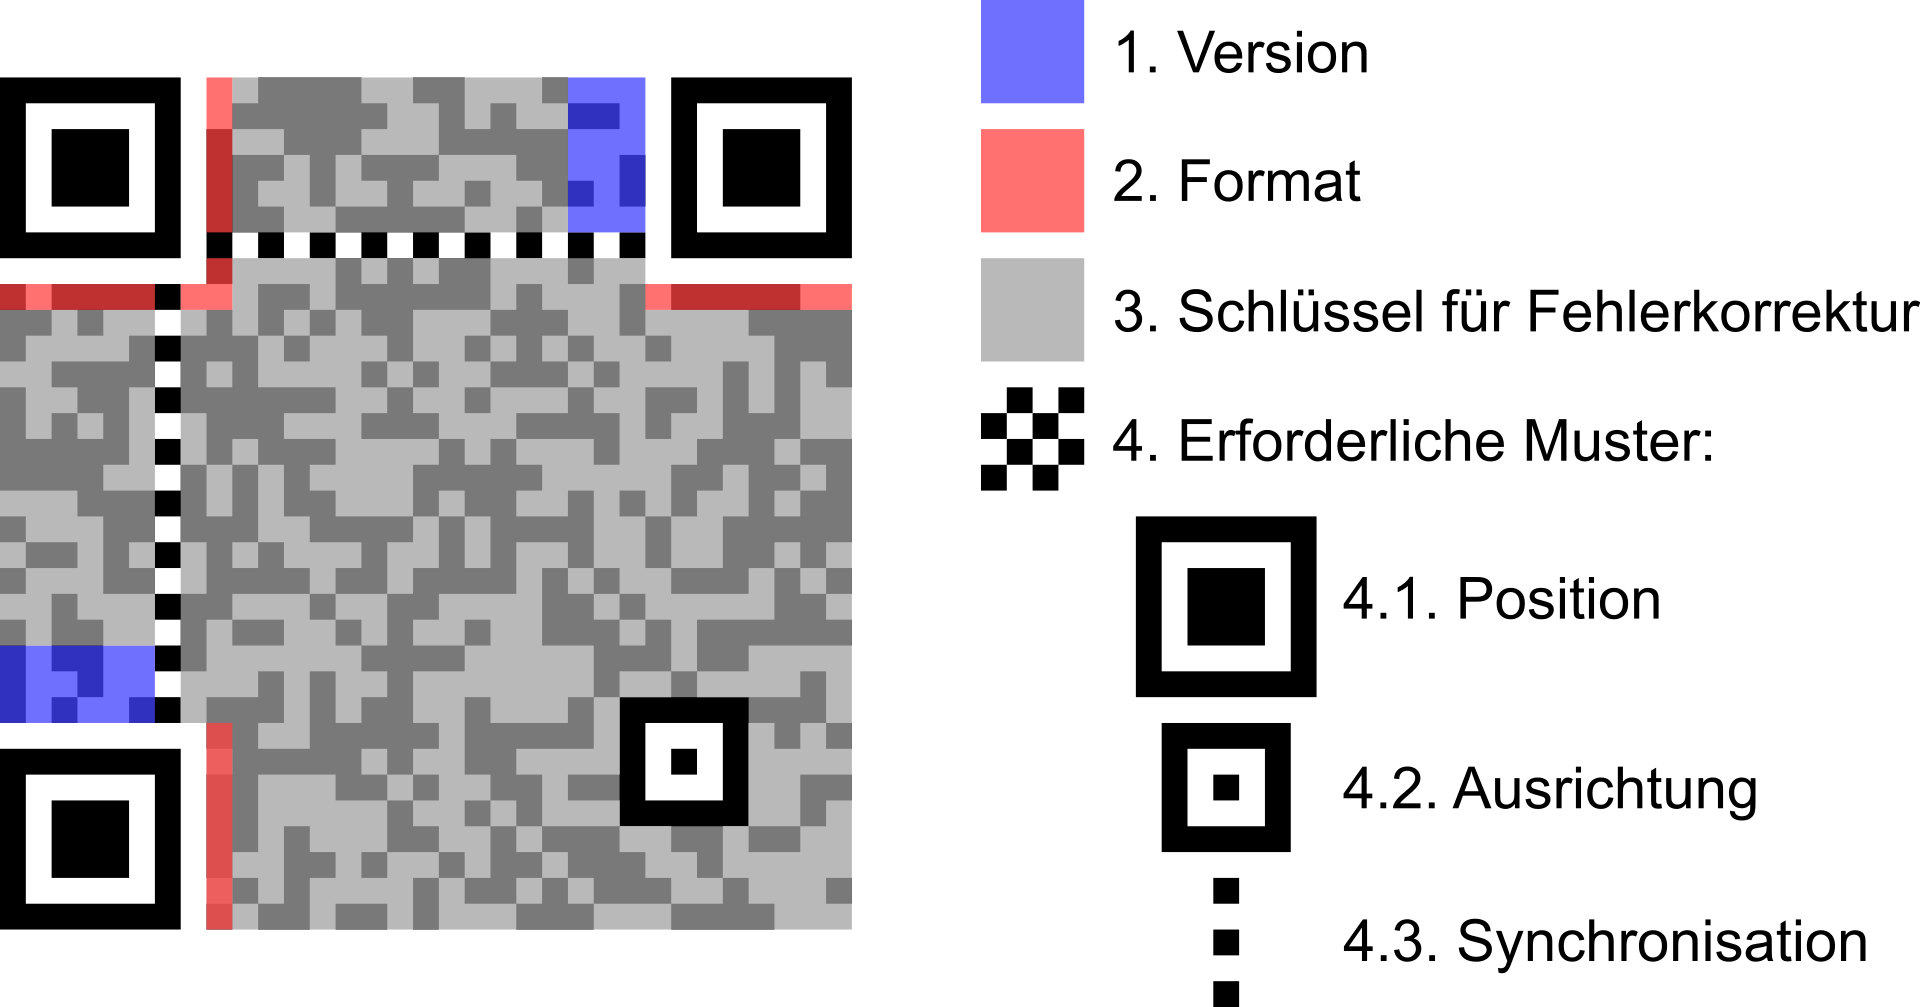
\includegraphics[scale=0.12]{pictures/QRCodeBild} 
 	\caption{QR-Code Struktur \cite{qrexapmle}}
\end{figure}

Ein QR-Code besitzt die Fähigkeit bis zu 4296 Alphanumerische Zeichen zu speichern. QR-Codes werden mehr im öffentlichen Rahmen benutzt, so werden diese für Kommerzielle Zwecke bei Werbungen, Webseiten, Plakaten und ähnlichem benutzt.

\subsection{Generierung}
\begin{enumerate}
\item Anhand der Länge des Textes und dem Grad der Fehlerkorrektur wird bestimmt, wie groß der QR-Code sein muss. 
\item Eine weißen Fläche wird erzeugt, auf der nach und nach alle Elemente des QR-Codes dargestellt werden. 
\item Die Erkennungsmuster, die nicht von dem Text abhängen, werden zuerst auf die Fläche gebracht. Das sind die Positionsmuster, die  Ausrichtungsmuster und die Synchronisationslinien.
\item Aus dem Text wird eine Bitfolge generiert.
\item Zu der Text-Bitfolge wird eine weitere Bitfolge für die Fehlerkorrektur generiert.
\item Die Text-Bitfolge wird zusammen mit der Fehlerkorrektur-Bitfolge dort in das Feld gezeichnet, wo noch Platz ist. Dies geschieht von rechts nach links in Schlangenlinien.
\item Um ungefähr gleich viele schwarze und weiße Pixel auf dem QR-Code zu generieren und um Muster zu vermeiden, werden nacheinander acht verschiedene Masken über das Symbol gelegt. Die Maske, welche das beste Ergebnis liefert, wird beibehalten.
\item Die Kennnummer der verwendeten Maske in das Bild gezeichnet.
\end{enumerate}

\newpage
\section{DataMatrix-Code}
Der DataMatrix-Code bekannter 2D-Code, welches älter als der QR-Code ist. Der äußere Ring zeigt an wie die Matrix einzulesen ist, zur Orietuerung sind zwei schwarze Balken auf der Linken und unteren Seite festgelegt. \cite{matrix}
Im Gegensatz zum QR-Code ist eine Fehlerkorrektur von bis zu 30\% möglich, es ist nicht möglich weniger als 30\% Fehlerkorrektur einzustellen. Für die Fehlerkorrektur existiert in Kombination mit einem Verfahren zur Fehlererkennung und zwei verschiedenen Verfahren zur Fehlerkorrektur. 
Ein DMC besitzt die Fähigkeit bis zu 2335 Alphanumerische Zeichen zu speichern. Im Gegensatz zum QR-Code wird der DMC in der Industrie verwendet um Komponenten zu markieren.

\begin{figure}[ht]
\centering   
	 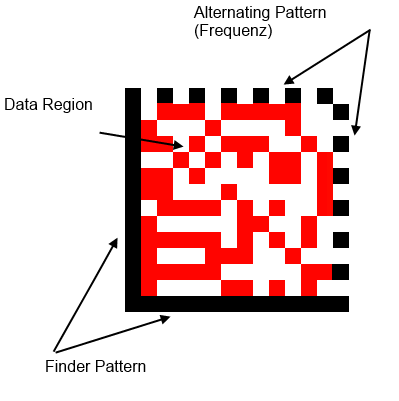
\includegraphics[scale=0.5]{pictures/dmc} 
 	\caption{DMC Struktur \cite{dmcexample}}
\end{figure}
\chapter{Konzept}
Das Hauptaugenmerk soll bei die Generierung und das Auslesen von QR-Codes liegen. Die Applikation soll aus einer Hauptseite bestehen welches zu den jeweiligen Activity Pages führt. Die Generation eines QR-Codes lokal in der Activity geschehen dazu soll ein Text eingebbar sein. Das Auslesen und Entschlüsseln der Informationen des QR-Codes, soll mithilfe der Smartphone Kamera ebenfalls direkt auf dem Endgerät stattfinden.
\chapter{Implementierung}	
Im Rahmen dieses Projektes wurden verschiedene Ansätze betrachtet um eine Android Applikation zu entwickeln. Eine eigene Implementierung des QR-Code Generierungsalgorithmus hätte zu viel Ressourcen gekostet. Deswegen wurde eine vorgefertigte Bibliothek \footnote{https://github.com/zxing/zxing} verwendet. 
\section{Generator}
Wie bereits erwähnt wurde für das Generieren in der Applikation eine externe Bibliothek verwendet, diese mach es dem User sehr einfach eigene Codes zu erzeugen. Die Bibliothek ermöglicht das Erstellen von DMC, Barcodes und QR-Codes, sowie das auslesen dieser Codes. In Abbildung 3.1 ist die Startseite der Applikation zu sehen, von dort aus kann man direkt auf die beiden Funktionen (Scannen und Generieren) zugreifen. In Abbildung 3.2 ist ein bereits generierter Code zu sehen. 
Um einen neuen Code zu generieren muss in das obige Textfeld ein Text eingegeben werden, nachdem auf den ``Generieren''-Button gedrückt wurde wird nach der Generierungsmethode wie in Absatz 2.1.1 beschrieben die Bitmap erstellt und angezeigt.
\newpage
\begin{figure}[ht]
\centering
   \begin{minipage}[b]{.4\linewidth} % [b] => Ausrichtung an \caption
	\centering
	 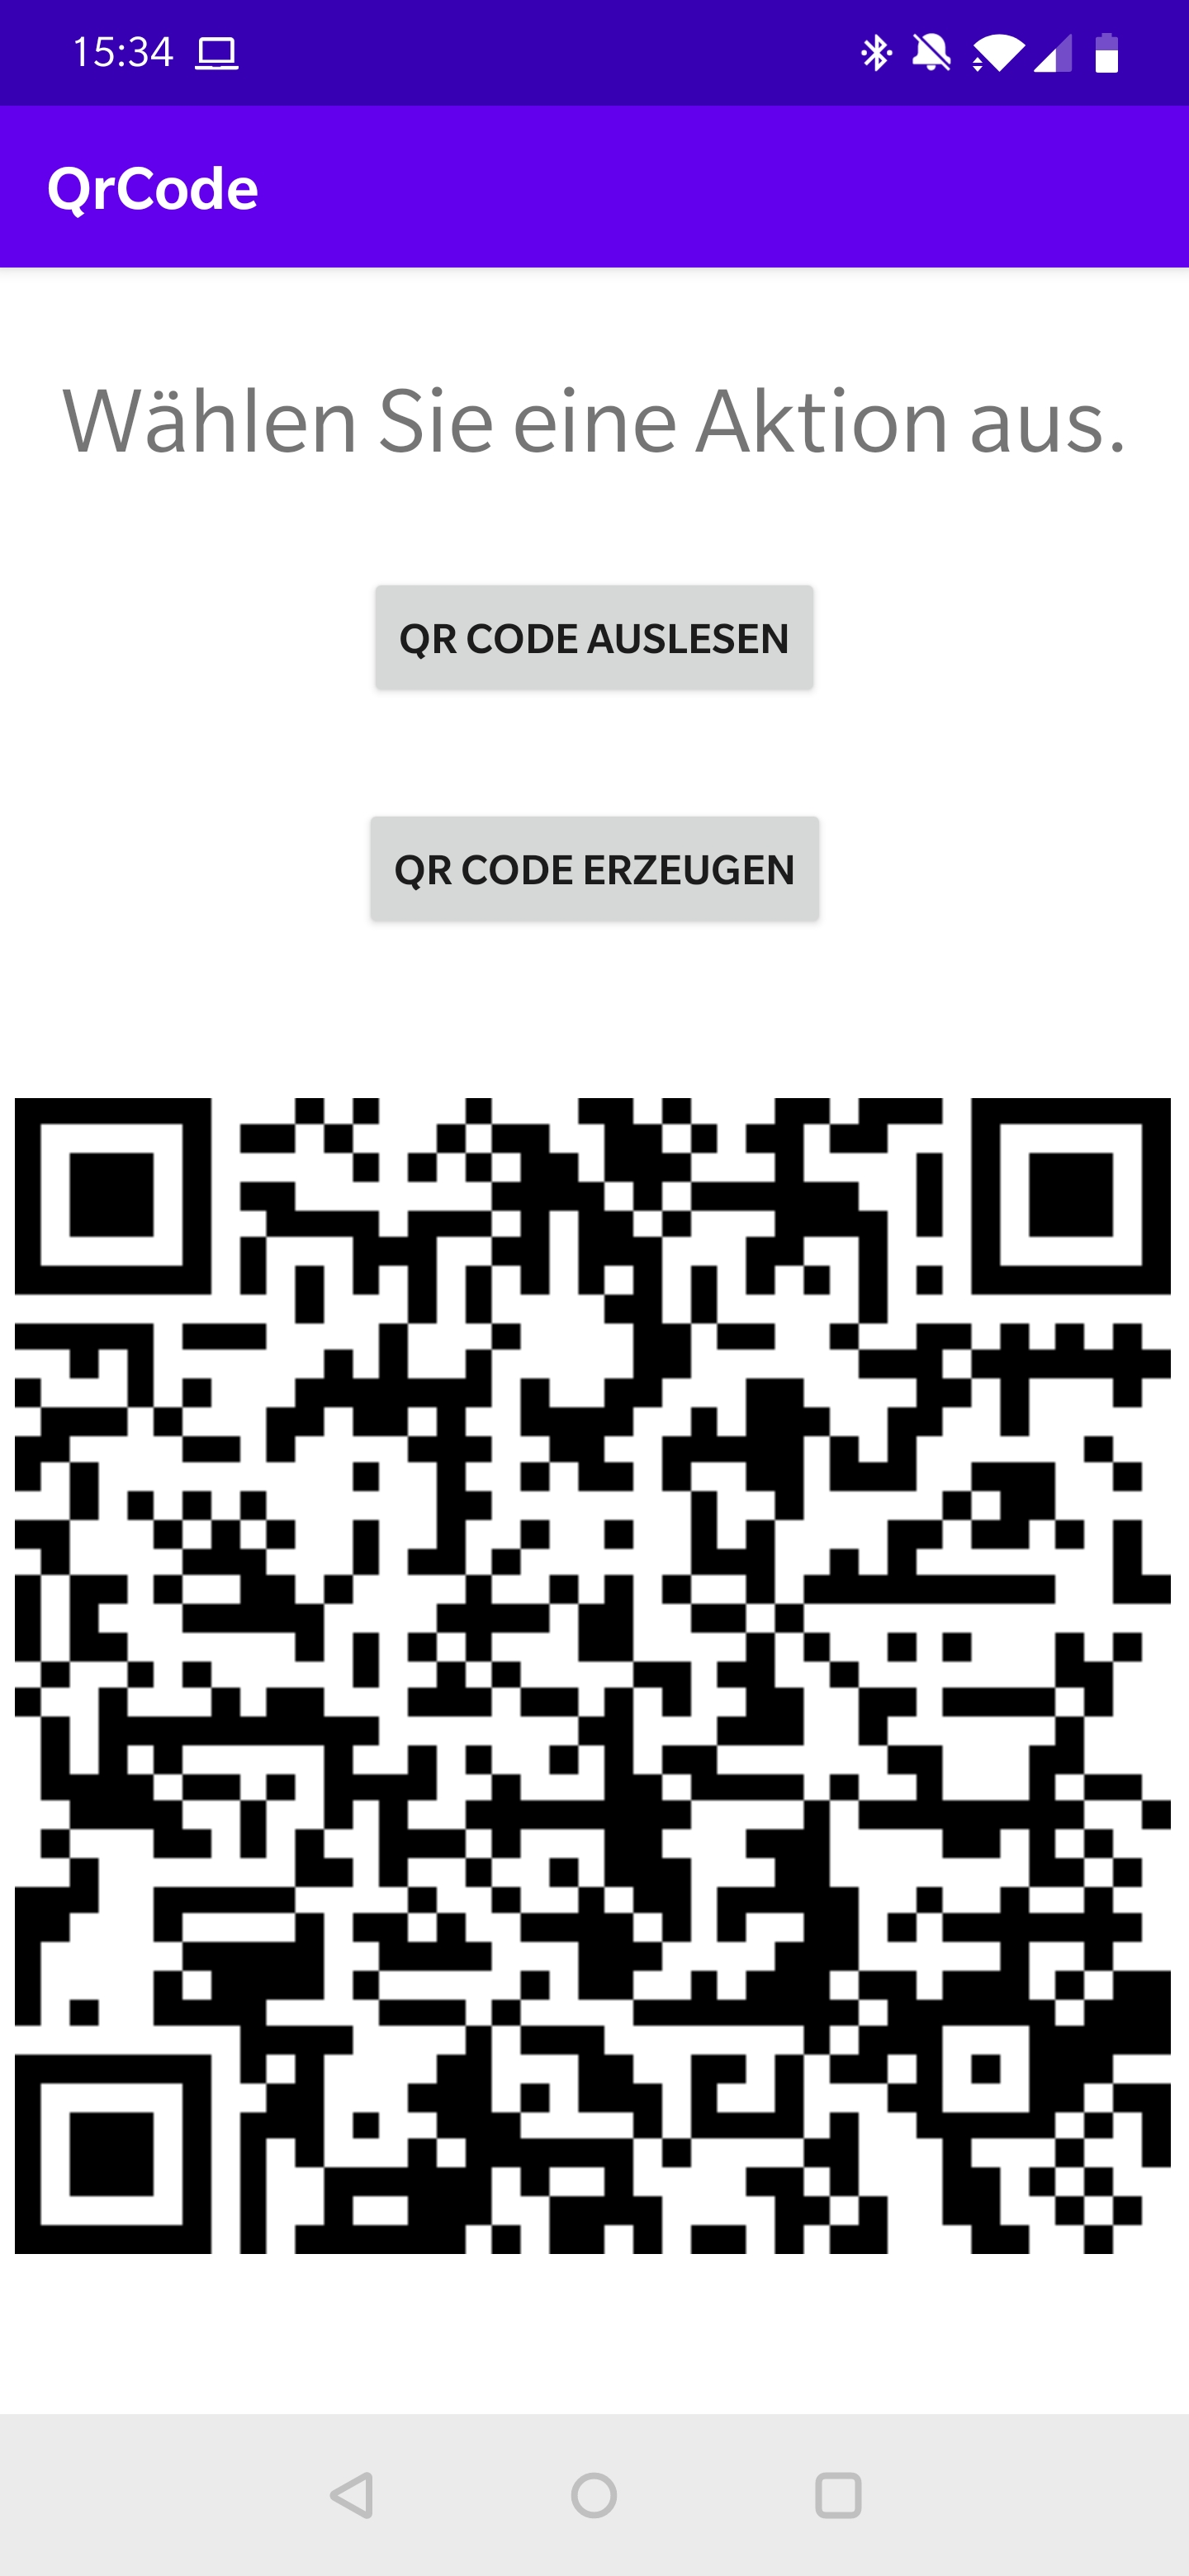
\includegraphics[scale=0.1]{pictures/MAIN} 
 	\caption{Main Activity}
   \end{minipage}
   \hspace{.1\linewidth}% Abstand zwischen Bilder
   \begin{minipage}[b]{.4\linewidth} % [b] => Ausrichtung an \caption
	\centering
	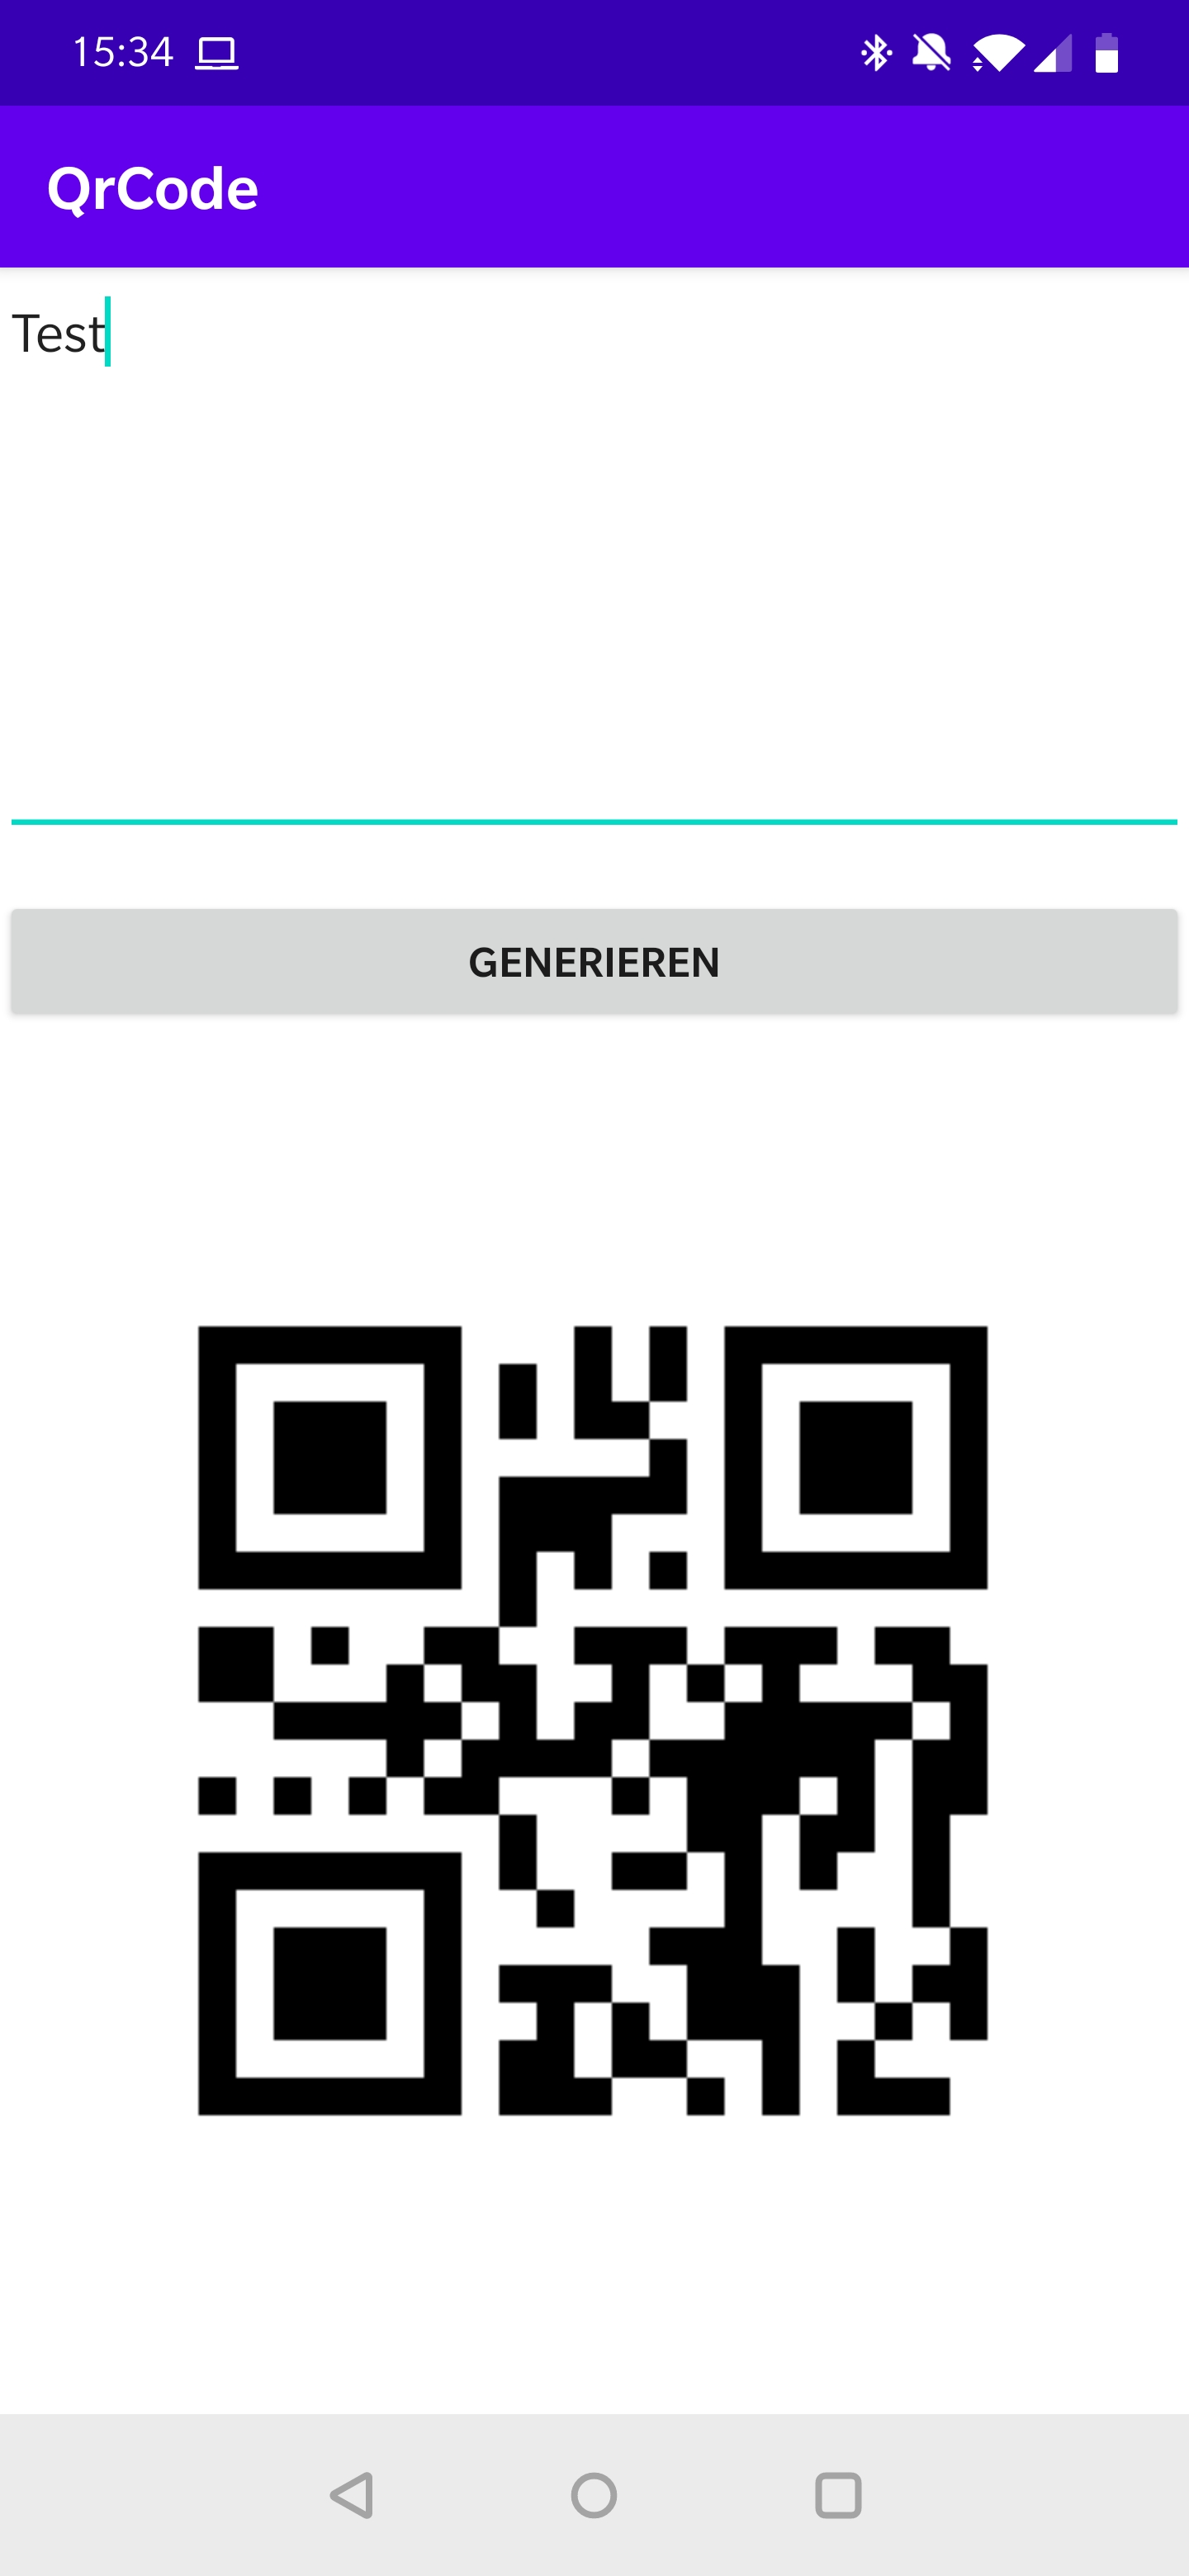
\includegraphics[scale=0.1]{pictures/Generate} 
	\caption{Generate Activity}
   \end{minipage}
\end{figure}
\newpage

\section{Auslesen}
Für das Auslesen wurde die gleiche Bibliothek wie für das generieren verwendet. Wie in Abbildung 3.3 ist zu sehen wie die Scan-Activity aussieht. Um ein QR-Code abzuscannen ist es nötig dieses vor das helleren Kästchen zu halten. Sobald dieses abgescannt wurde, erklingt ein Scanton und ein Popup mit dem Inhalt des Codes wird angezeigt. Handelt es sich um eine Webseite steht kann diese durch einen einfachen Knopfdruck besucht werden. Sind die beinhalteten Daten reine Informationen so werden diese nur dargestellt. Dies soll dem Nutzer die Möglichkeit bieten vor dem weiterleiten, eine Selbsteinschätzung abzugeben ob diese Webseite vertraulich ist.
\begin{figure}[ht]
\centering
   \begin{minipage}[b]{.4\linewidth} % [b] => Ausrichtung an \caption
	\centering
	 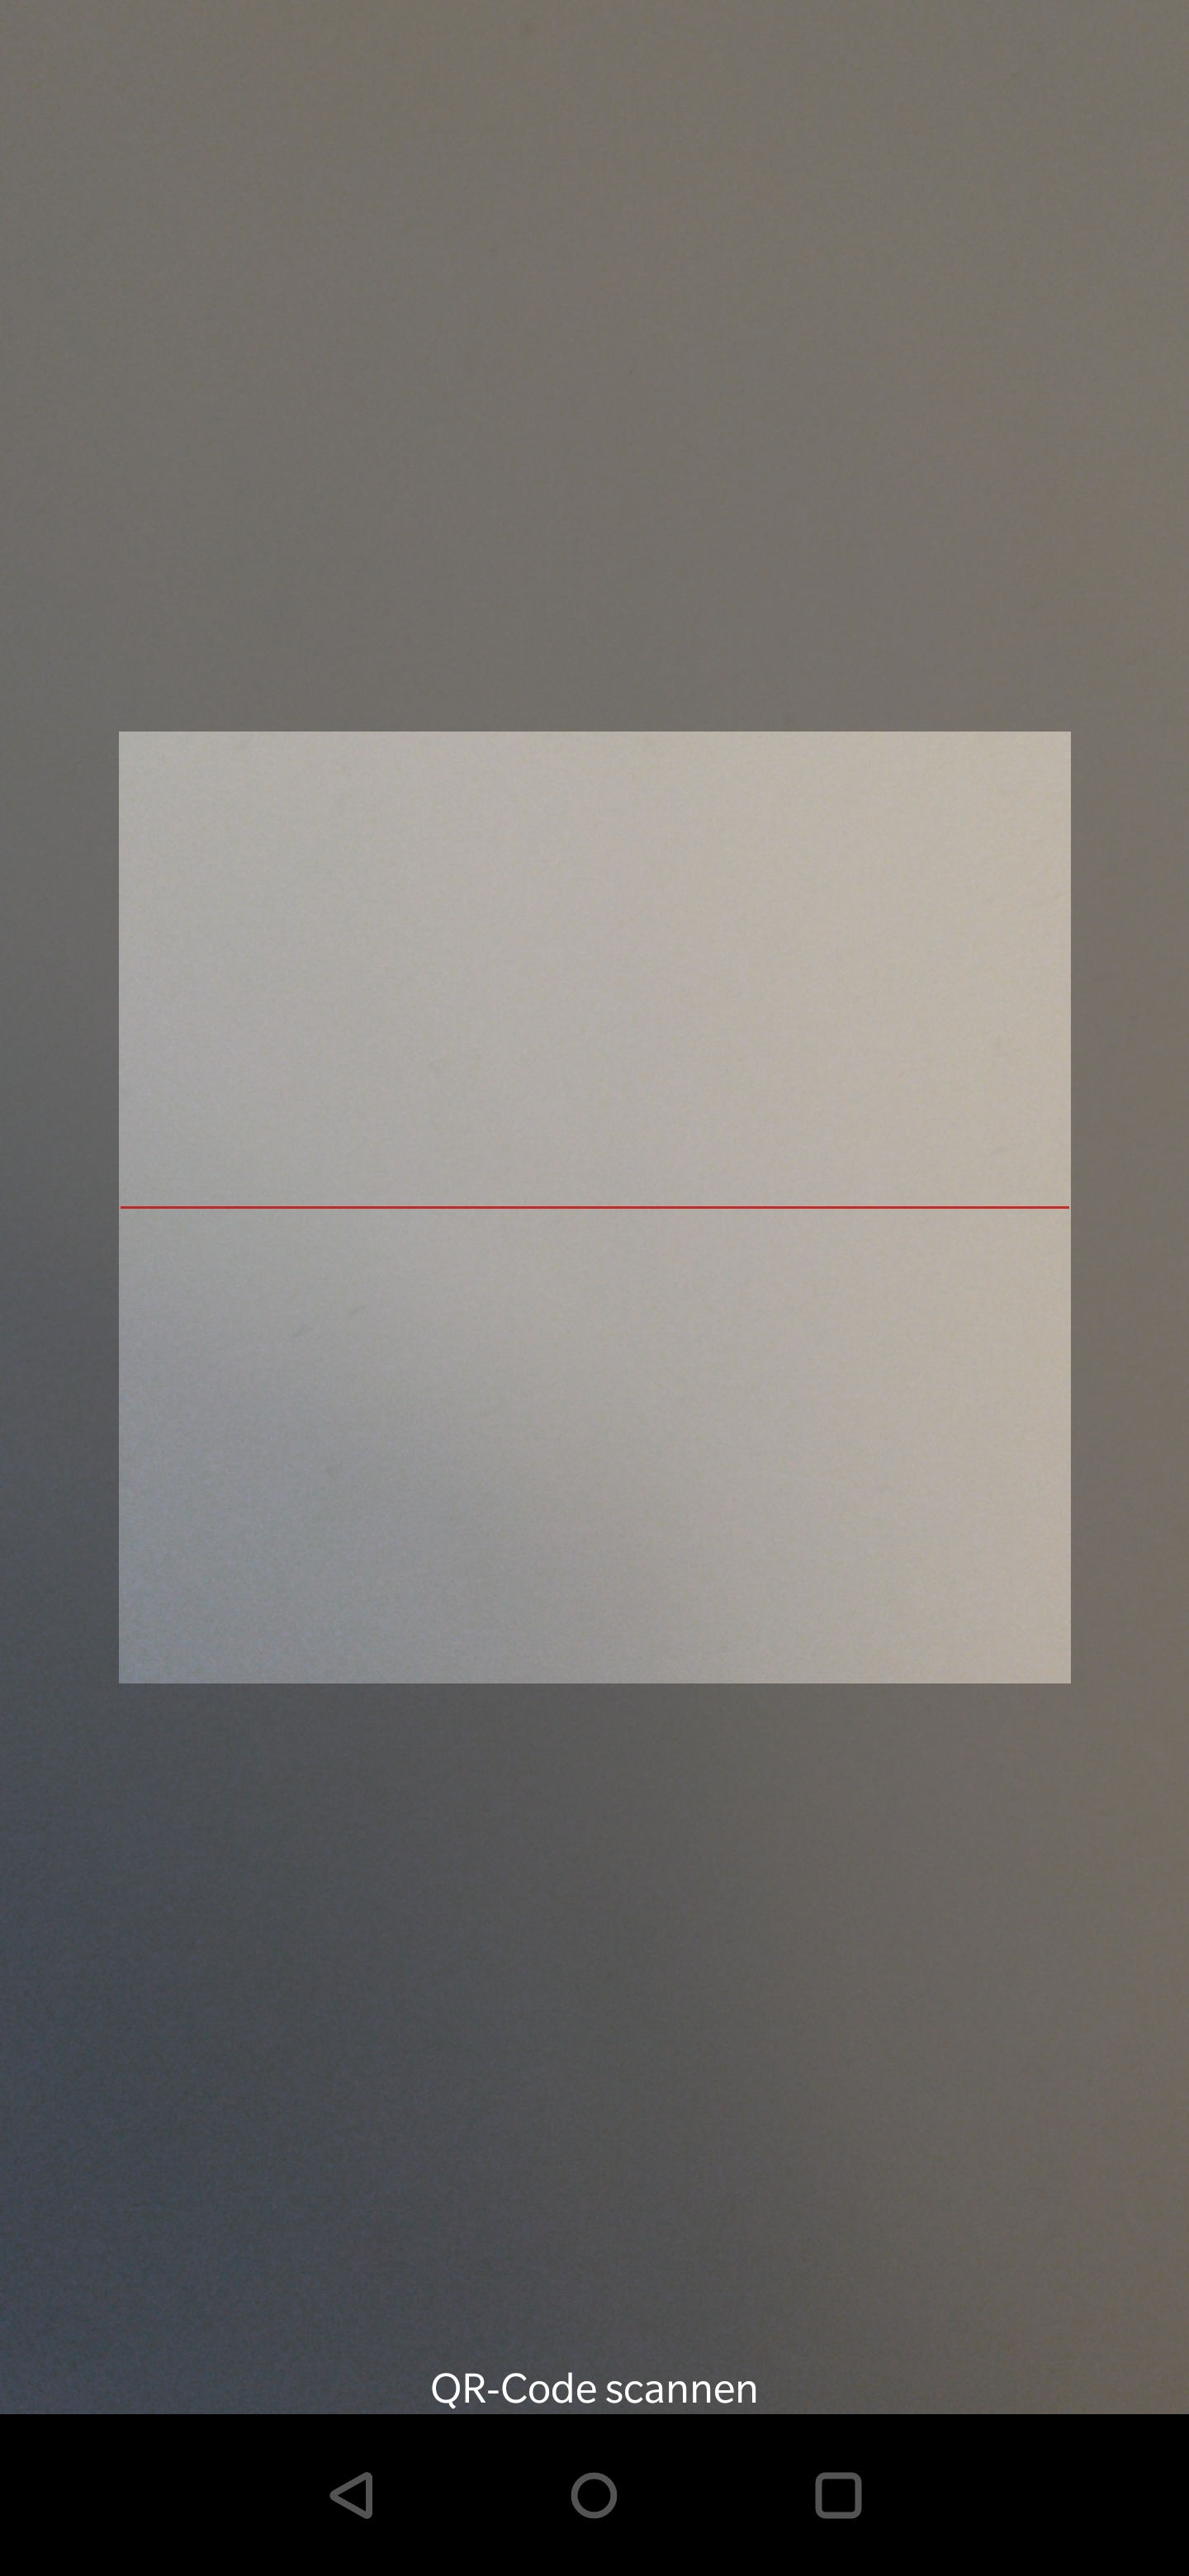
\includegraphics[scale=0.1]{pictures/scan} 
 	\caption{Scan Activity}
   \end{minipage}
   \hspace{.1\linewidth}% Abstand zwischen Bilder
   \begin{minipage}[b]{.4\linewidth} % [b] => Ausrichtung an \caption
	\centering
	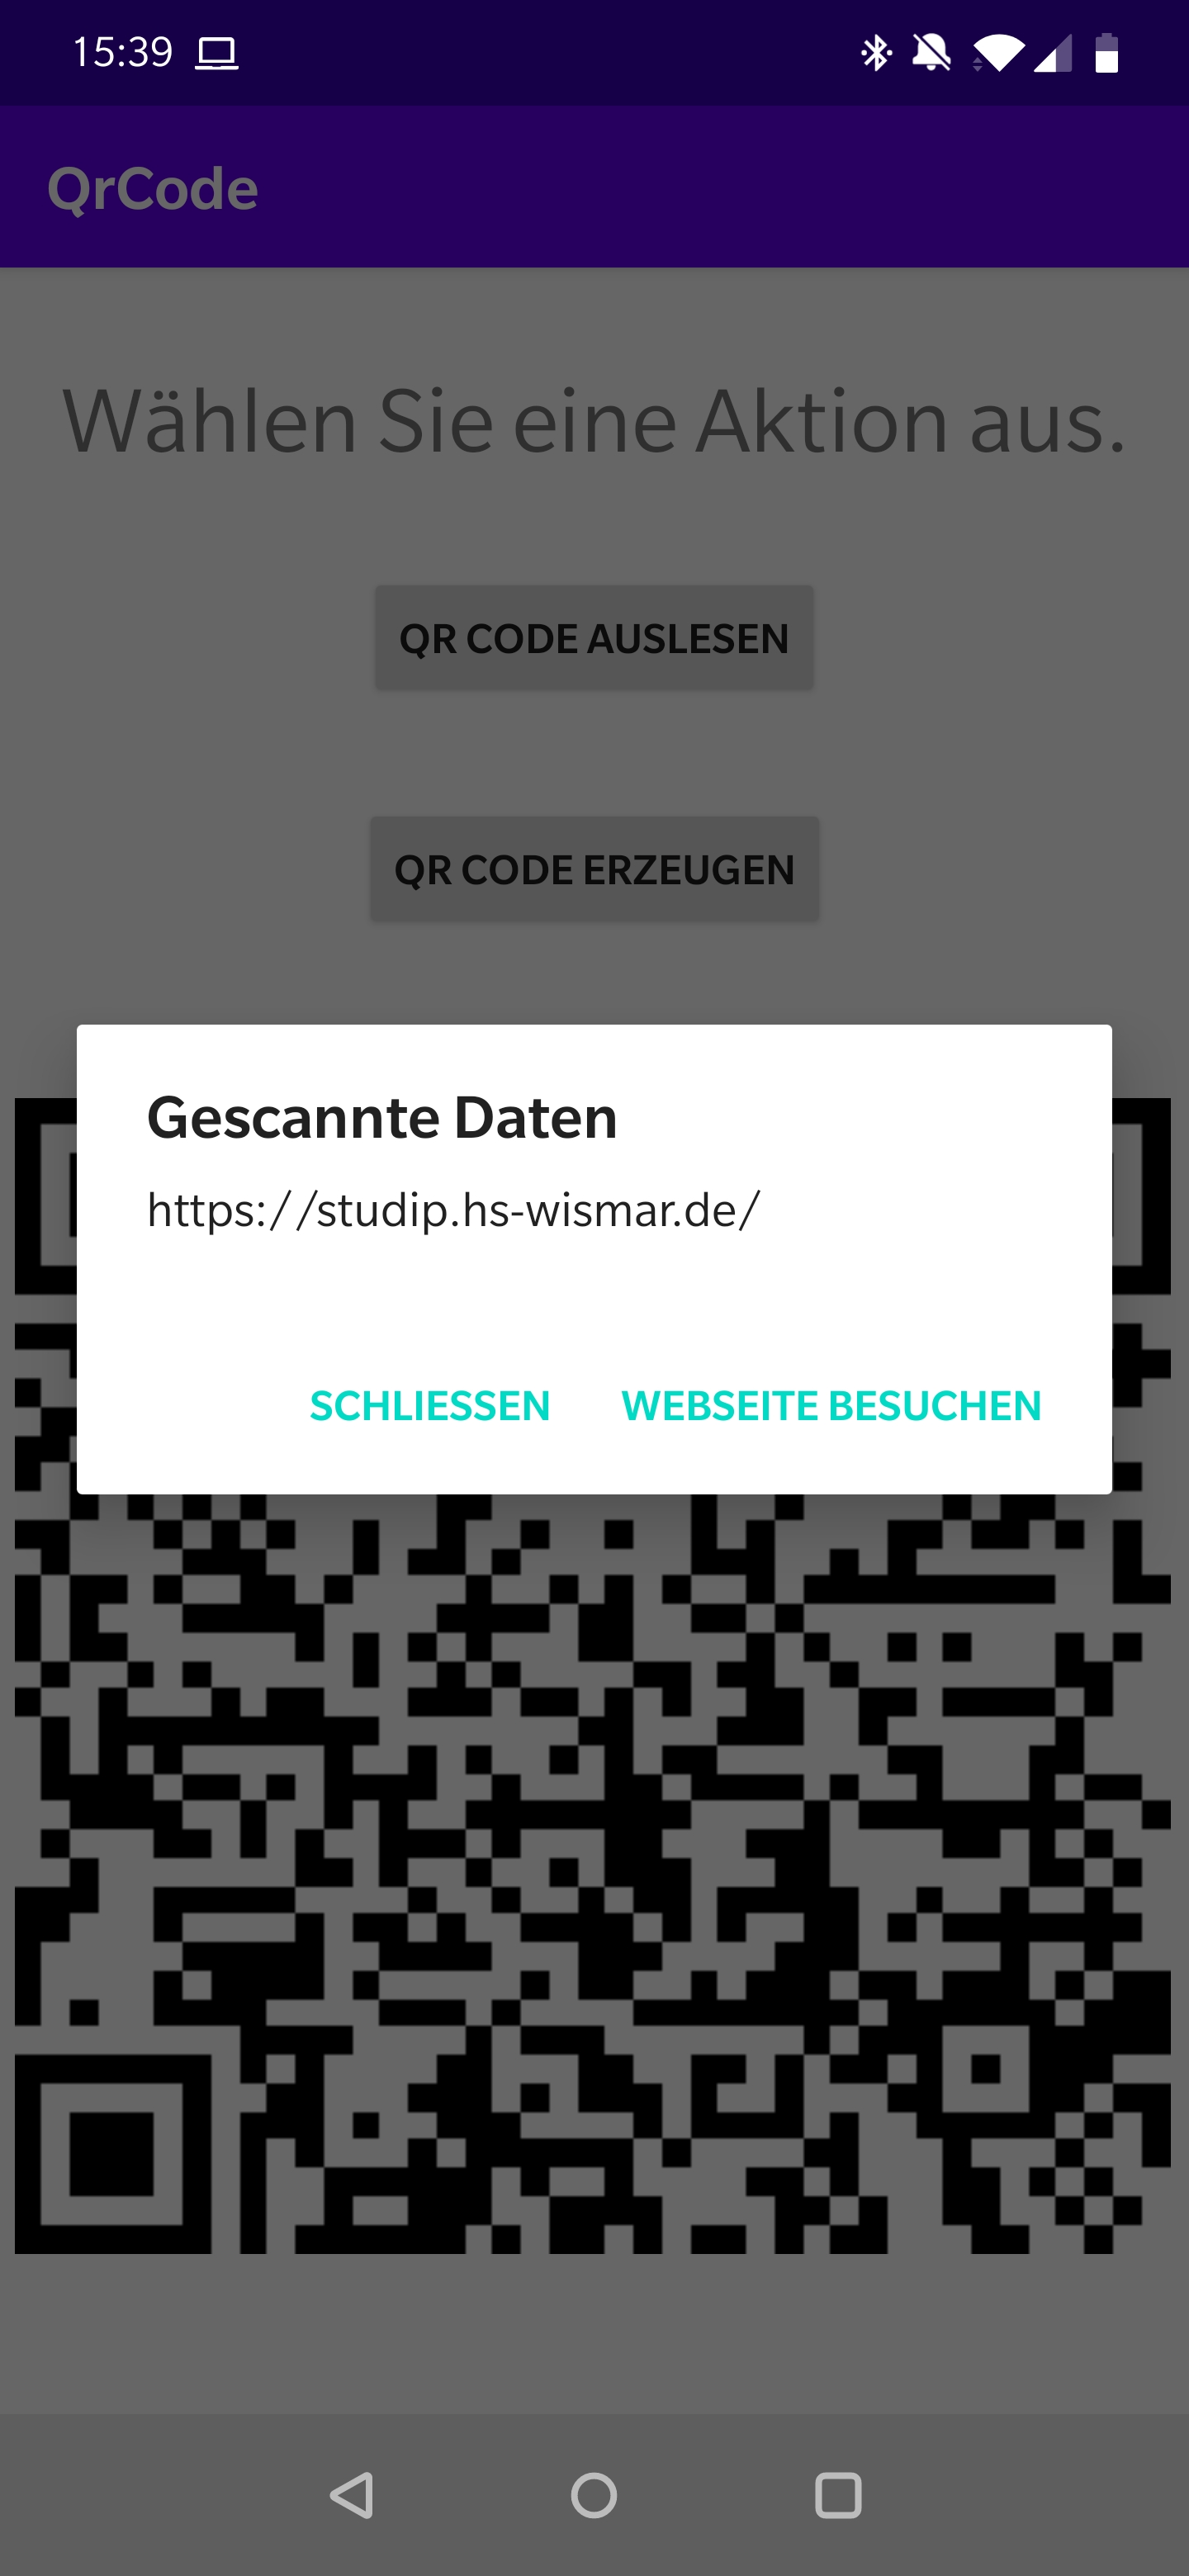
\includegraphics[scale=0.1]{pictures/popup} 
	\caption{Scan PopUp}
   \end{minipage}
\end{figure}
\newpage
\chapter{Schlussfolgerung}
Gegenüber dem DMC ist der QR-Code weitaus mehr bekannt und besitzt eine Etablierte Rolle, dadurch sind QR-Codes im Rahmen der Werbung sehr Wertvoll und bieten dem Ersteller und Verteiler die Möglichkeit mit wenig Aufwand viel Traffic zu erreichen. 
Durch vorgefertigte Implementierungen ist es sehr einfach für eigene Projekte solche Codes zu generieren. 

Während der Ausarbeitung dieses Projektes gab es noch keine Signifikanten Hinweise auf einen Nachfolger des QR-Codes. 






\pagenumbering{roman}

	%-----------------------------------------------------------------------------
	% Literaturverzeichnis einf�gen, 
	% Nutzung der BibTeX-Technologie --> literatur.bib 
	%-----------------------------------------------------------------------------

	
	\bibliographystyle{unsrtdin}		%  Stil des Literaturverzeichnisses (hier nach DIN 1505)
	\bibliography{literatur}			% gibt Datei mit der Literatur an
	
	\nocite{*}						% damit alle in der DB enthaltende Eintr�ge bearbeitet werden
	

	%-----------------------------------------------------------------------------
	% Verzeichnisse
	%-----------------------------------------------------------------------------
	\listoffigures						% Bildverzeichnis einf�gen

	%-----------------------------------------------------------------------------
	% Anhang
	%-----------------------------------------------------------------------------	
	\appendix
	% Auch hier sind Gliederungen aller \chapter, \section
	

	%-----------------------------------------------------------------------------
	% Selbstst�ndigkeitserkl�rung
	%-----------------------------------------------------------------------------	
	\chapter*{Selbstst\"andigkeitserkl\"arung}
	\addcontentsline{toc}{chapter}{Selbstst\"andigkeitserkl\"arung}
	\rhead{Selbstst\"andigkeitserkl\"arung} % rechts oben in der Kopfzeile Chapter darstellen
	Hiermit erkl\"aren wir, dass wir die hier vorliegende Arbeit selbstst\"andig,
	ohne unerlaubte fremde Hilfe und nur unter Verwendung der aufgef\"uhrten
	Hilfsmittel angefertigt haben.

	\begin{tabular}{p{10cm}p{13cm}}
		\\
  		\\
  		\\
  		\\
  		Wismar, den \today \\
  		---------------------------------------  & ------------------------------ \\
  		Ort, Datum & Unterschrift
	\end{tabular}
	

\end{document}							% Ende des Dokuments
%-----------------------------------------------------------------------------
%quelle : http://www.datamatrixcode.net/data-matrix-code-vs-qr-code/ https://de.wikipedia.org/wiki/Datei:QR_Code_Struktur_Beispiel.svg 8.7.2020
